\documentclass[10pt]{book}
\usepackage[utf8]{inputenc}
\usepackage[italian]{babel}
\usepackage{multicol}
\usepackage[bookmarks]{hyperref}
\usepackage[a4paper, total={18cm, 25cm}]{geometry}
\usepackage{listings}
\usepackage{graphicx}
\usepackage{makecell}
\graphicspath{ {./img/} }
\usepackage{color}

\begin{document}
\renewcommand*\contentsname{Indice}
\title{Gestione di Reti}
\author{Federico Matteoni}
\date{A.A. 2019/20}
\maketitle
\tableofcontents
\pagebreak
\section*{Introduzione}
\paragraph{Perché bisogna studiare la gestione?} La situazione corrente comprende: un aumento delle risorse strategiche informative, le reti di computer che da strumento di supporto sono diventate elemento chiave delle organizzazioni, l'aumento esponenziale dei dispositivi interconnessi e aumento anche della complessità e delle funzionalità.\\
C'è quindi richiesta di servizi di rete permanenti e di qualità ottimale, oltre alla necessità di ridurre i costi per le infrastrutture di rete di un'azienda.
\paragraph{Necessità} Gestione di reti eterogenee con l'aiuto dei computer.
\section*{Terminologia e concetti fondamentali}
\paragraph{Managed Objects} Il controllo, la coordinazione e il monitoraggio delle risorse avviene tramite la manipolazione dei cosiddetti \textbf{managed objects}: un MO è una visione astratta di una risorsa che presenta le proprietà dal punto di vista della gestione. Sono \textbf{rappresentazioni astratte di risorse reali}.\\
I confini di un MO specificano quali dettagli sono accessibili ai sistemi di monitoraggio e quali sono schermati (\textbf{black box})

\begin{center}
Management-System $\leftrightarrow$ Managed Object $\leftrightarrow$ Real Object
\end{center}
\begin{list}{}{\textbf{Caratteristiche}}
	\item \textbf{Attributi}: descrivono lo stato/condizione dell'MO, possono cambiare quando cambia lo stato dell'oggetto reale e possono essere manipolati attraverso operazioni di management
	\item \textbf{Operazioni}: consentono l'accesso all'MO. Operazioni tipiche sono get, set, create e delete, ma il numero e tipo delle operazioni influenzano perfomance e complessità dell'oggetto
	\item \textbf{Comportamento}: determina la semantica e l'interazione con la risorsa reale. Normalmente definito in linguaggio naturale
	\item \textbf{Notifiche}: quantità e tipologia dei messaggi, che possono essere generati da situazioni pre-definite da un MO quando avviene una specifica situazione
\end{list}
\paragraph{Management Information Base} L'unione di tutti i MO contenuti in un sistema forma la MIB del sistema. La \textbf{Management Information Base} è la collezione di tutti i management object all'interno del sistema, con i loro attributi.\\
Una MIB deve essere conosciuta sia da chi la implementa che da chi la gestisce.
\subparagraph{Modularità} Gli MO di un sistema sono solitamente definiti in più MIB. Nelle MIB sono introdotti i moduli per consentire un design modulare: moduli diversi possono essere definiti da team diversi, le funzionalità di gestione possono essere estese e modificate\ldots
\paragraph{Paradigma Gestore/Agente}
\begin{list}{}{Agent}
	\item Implementa i MIB delle MO accedendo alle risorse reali
	\item Riceve le richieste da un gestore, le processa e trasmette le risposte appropriate
	\item Smista le notifica riguardanti cambiamenti di stato importanti nel MIB
	\item Protegge gli MO da accessi non autorizzati usando regole di controllo degli accessi e autenticazione della comunicazione
\end{list}
\begin{list}{}{Manager}
	\item Esercita il controllo delle funzioni
	\item Avvia operazioni di gestione tramite opportune operazioni del protocollo per la manipolazione degli MO
	\item Riceve messaggi dagli agenti e li inoltra alle applicazioni interessate per la gestione
\end{list}
\paragraph{Management Protocol} Un protocollo di gestione implementa l'accesso a MO distanti attraverso la codifica di dati di gestione (management data)
\section{lezione 2}
Livello 2 consente di identificare un device sulla rete. In tutte le reti c'è la necessità di identificare la porta di rete. Ogni dispositivo ha almeno un'interfaccia di rete: loopback, che consente di far comunicare processi di rete sulla stessa macchina. \texttt{127.0.0.1} consente di parlare su stessa macchina senza trasmettere sul filo, fondamentalmente un cortocircuito.\\
\texttt{ifconfig} consente di vedere le interfacce di rete disponibili su unix.\\
Se si vuole gestire una rete è fondamentale la standardizzazione.\\\\
Output \texttt{ifconfig}. Parte degli indirizzi, no indirizzo hw su loopback perché il traffico non esce mai (loopback sulla pila OSI è nel livello 3 Network, il MAC address è sul livello 2 Data Link, che non viene toccato da loopback). Indirizzo MAC 6 byte divisi in blocchi dai due punti. I primi 3 identificano il costruttore della scheda di rete. I successivi tre identificano la scheda di rete per il costruttore, che lo setta univocamente. Ciò garantisce univocità. Per primo blocco di tre ho 16M di dispositivi possibili. I MAC address quindi \textbf{non sono univoci}, lo sono \textit{probabilmente}. L'univocità è fondamentale sulla stessa rete. Quindi indirizzo hw identifica univocamente device sulla rete locale. divisi in due blocchi, il primo identifica costruttore della scheda di rete.\\\\
Qualsiasi dispositivo ha indirizzo hw diverso per ciascuna porta.
\section{Ethernet}
Ethernet è un cavo seriale, trasmissione e ricezione. Mezzo seriale. Un filo.\\
Quando si mandano dati non posso tutti insieme ma man mano. Non c'è collisione perché ricezione e trasmissione sono su due fili separati.\\
Pacchetti inviati nel tempo sul filo. Vengono distinti tra loro dal \texttt{preamble}. Pacchetti inviati in una direzione: preambolo, destinazione, sorgente, tipo dei dati, dati effettivi, padding (per rendere pacchetto di 64 se pacchetto è troppo corto), CRC.\\
Quindi per spedire pacchetto necessito di indirizzi (chi voglio e chi sono) e cosa mandare. chi sono lo so, è scritto nella scheda. Voglio conoscere indirizzo di chi voglio.\\
Alla connessione del cavo, se DHCP manda fuori pacchetto per richiesta quindi switch lo impara, se IP statico manda pacchetto ARP quindi switch lo impara.\\
MAC address randomizzato per privacy, spesso e volentieri sui dispositivi mobili.\\
Possibile più di un utente sulla stessa rete con soliti indirizzi, apparati avanzati se ne accorgono.
\section{lezione 3}
un pacchetto è interamente creato dal computer, quindi "non ci si può fidare"\\
Bisogna andare a livello fisico e autenticare, un po' come chiedere la carta d'identità. Metter in atto meccanismi che impediscano di inibire riconoscimento della sorgente.\\
802.1x permette di entrare in rete. Se configurato, il device prima di entrare in rete espone delle credenziali (utente, password, protocollo autenticazione\ldots)\\
Da quel momento in poi \textbf{allegato} al pacchetto c'è il mio nome, ma le informazioni di autenticazione non fanno parte del pacchetto: pacchetti creati quando non c'era preoccupazione e interesse in fattori di sicurezza delle trasmissioni.\\
L'informazione non è parte del pacchetto ma lo riconosce in qualche altro modo il device e \textbf{rimane nel device} (Access Point). Ciò non serve per autenticazione fisica sul cavo: so che sei tu su questo cavo. Ma è necessaria per autenticazione su mezzi condivisi (wifi).\\
Su router MAC cambia ad ogni hop (ethernet comunicazione punto-punto), IP cambia solo se c'è NAT. Le parti da lv 3 in su non cambiano (a meno di frammentazioni\ldots)\\
Robustezza delle reti si fa tramite la ridondanza. Tipico mettere più strade per spedire il traffico: load balancing.\\
Vale sia per corrente elettrica che per traffico di rete.\\\\
\subsection{Aree funzionali}
FCAPS per gestire \textbf{qualsiasi sistema}, da giochi a sistemi di rete. Non sono mutualmente indipendenti.
\begin{list}{}{}
	\item \textbf{Fault Management}: error detection, isolation and repair\\
	Se qualcuno rileva malfunzionamento (riempito disco, ram, sovraccarico CPU\ldots) lo deve notificare
	\item \textbf{Configuration Management}: devo sapere com'è configurato il sistema. Leggere la configurazione è importante, così che le app si possano basare sulle API comuni e funzionare correttamente. Fondamentale capire la configurazione perché permette di definire l'amministrazione, servizi\ldots, possibile riconoscere anche le adiacenze e "questo filo qui va su questa porta qua". che impatto ho se stacco questo cavo, o si rovina? Informazioni sufficenti per amministrare la rete
	\item \textbf{Account Management}: rilevare il consumo di risorse
	\item \textbf{Performance Management}: efficenze e statistiche, performance di sistema sia lato utente sia lato fornitore. Per l'utente è riuscire ad usare la rete, per l'operatore è il giusto compromesso tra investimento sul mezzo e contentezza utente.
	\item \textbf{Security Management}: assicurarsi che ciò che uno fa è effettivamente possibile farlo, autoproteggendosi perché con le reti odierne posso intasare rete (volente o no) e quindi intasare internet, provocando danni
\end{list}
\subsection{Interagire con management object}
Primitive: get, set, create, delete\\
Quando faccio richiesta ad un protocollo mi aspetto una risposta: richiesta -- risposta\\
Contenuto richieste varia durante il transito aggiungendo determinate informazioni. Es: SMS durante il transito aggiunge numero mittente per poter comunicare a destinatario chi inviava.
\subsection{Servizi}
\paragraph{Confermati} Faccio richiesta $\rightarrow$ mi aspetto risposta.\\Es: Telegram/Whatsapp
\paragraph{Non confermati} Faccio richiesta e fine.\\Es: SMS
\begin{center}
	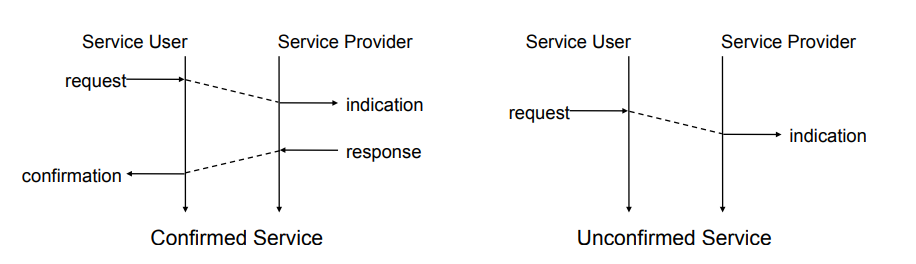
\includegraphics[scale=0.7]{timediag.png}
\end{center}
\subsection{Standardizzazione}
La grande differenza tra ISO/OSI e Internet è il processo di standardizzazione.
\pagebreak
\paragraph{ISO} Nella standardizzazione ISO tutte le varie aziende si accordano su come fare la rete: si creano gruppi di lavoro che si riuniscono (es. ICANN) e producono un documento di lavoro, poi vari comitati lo discutono (fino a qui \textbf{ad alto livello}).\\
Se si mettono d'accordo, pubblicano un \textbf{Draft International Standard} (\textbf{senza implementazione}). Dopodiché, se non viene accettato, creano technical report oppure un \textbf{full standard}.\\
La parte importante è l'assenza di implementazione fino ad avere la creazione dello standard.

\begin{center}
	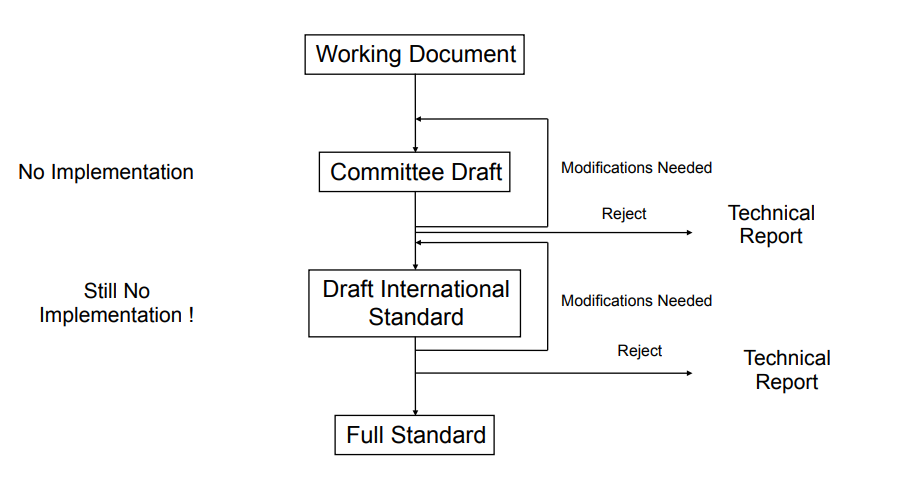
\includegraphics[scale=0.7]{stdiso.png}
\end{center}
\paragraph{Internet} Nella standardizzazione internet è tutto seguito dal comitato IETF, che pubblica aree d'interesse in cui ritiene ci sia possibilità di sviluppo. La sottomissione di un'idea ad un'area d'interesse è libera, oppure si può mandare una mail per idee completamente nuove. Dal working document a draft passa poco e i draft dopo pochi mesi scadono. Dopo massimo due anni o si rifiuta o si fa il draft standard (draft RFC) che o lo si rifiuta o diventa standard in max 4 anni. Necessita di più implementazioni interoperabili.
\begin{center}
	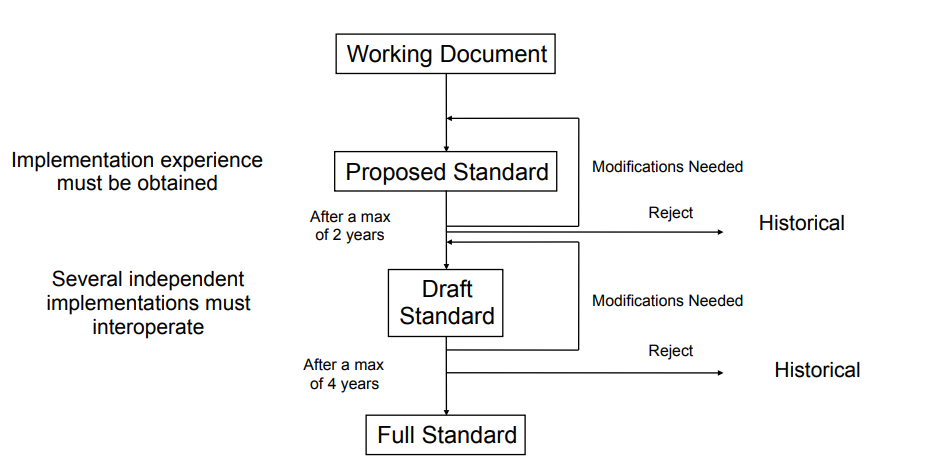
\includegraphics[scale=0.7]{stdietf.png}
\end{center}
\section{Abstract syntax notation one}
\paragraph{ASN1} Sintassi per la definizione di strutture dati e formato di messaggi. Ha l'obiettivo di consentire a macchine dalle differenti architetture hardware di scambiare dati, essere language neutral e consentire la negoziazione della codifica di trasmissione.\\
Come spostare le informazioni? Vari costruttori all'inizio lo facevano "in casa" senza interoperabilità. Col tempo si è reso necessario costruire qualcosa per scambiare le informazioni in maniera interoperabile.
\paragraph{Endian} Come si ordinano i dati in spedizione, per sapere qual è il più significativo.\\
Bit più significativo a sx è big-endian, ormai poco usato. Altrimenti è little-endian.
\section{lezione 4}
Nel monitorare il traffico di rete c'è il problema di come riceverlo. Non sempre siamo nel posto giusto. Se voglio vedere cosa fa altro dispositivo/sottorete a livello di traffico, come faccio? Opzioni: o possiamo mettere la mano sul pc (wireshark) o posso fare finta di essere il pc (chiedendo allo switch, non intrusivamente, di mandare il traffico verso pc pure a me) Prima di iniziare a guardare il traffico, il traffico va visto.\\
\subsection{Common problems with packet capture}
\ldots\\
Perché \texttt{root}? Perché scavalco ciò che fa un'applicazione, perché vedo tutto il traffico indipendentemente dall'applicazione. Per questo devo essere root.\\
Container condivide kernel con host, macchina virtuale emula il kernel.\\
Necessità vedere traffico. Non vorrei mettere mano sulla macchina, perché devo avere so che permette, utente, installare software\ldots\\
Quindi lo faccio da fuori, prelevandolo dallo switch.\\
Metodi software: ho switch, che ha delle porte:
port mirror: tutto traffico diretto verso tale macchina oltre a mandarglielo lo mandi anche a me su questa porta. 1:1 una porta verso una porta, 1:N tot porte switch le mandi qua.
VLAN mirror: simile al port mirror: dammi tutto traffico tale VLAN e mandalo qua
traffic filter/mirroring: dammi solamente traffico di tale porta tale ip\ldots\\\\\\
Singolo cavo ha 2gbps (1gps in upload e 1gbps in dwnld), quindi con port mirror, che posso scaricare al massimo a 1gbps, ho efficacia se traffico sta solo a 1gbps. Dovrei avere scheda di rete da 10gbps per reggere comodamente traffico e non perderlo. Scheda direte più veloce della somma delle due direzioni.\\
Hardware: Network Tap prende le singole direzioni del traffico e ne fa una copia. PC monitor con due schede di rete perché tap divide il filo le direzioni: una prende le direzioni in entrata e una prende la direzione in uscita. Così scopro anche chi invia cosa. Nel port mirror non sono preservate le direzioni.
\section{Lezione}
Software di switch e infrastruttura di rete devono essere duraturi, perché infrastruttura di rete si cambia quando c'è veramente necessità. Altrimenti infrastruttura rimane lì. 
\paragraph{Problema} Gestire le cose nel tempo, che rimangano interoperabili negli anni. Siccome informatica va avanti per mode, si sono posti come problema (fatta negli anni '80) dover gestire qualche sistema non attraverso la url come si fa ora, perché è un modo di fare molto volatile che cambia spesso. Allora hanno fatto standard con negoziazione alto livello: oggetto ha attributi ad alto livello, funzionali al suo funzionamento (macchinettà caffè: c'è acqua, quanti caffè fatti, se ha bicchierini\ldots).\\
Attributi, cosa ti mostro io che sia rilevante per te (non quante viti ha, ma lo stato), operazioni che si possono fare su quegli attributi (accendi, spegni\ldots), comportamento. Software si occupa dell'accensione, non so com'è fatto internamente, io mi limito a chiamare l'operazione. Standardizzazione di funzionamento.
\paragraph{Manager} Comanda l'operazione, impone politica di gestione.
\paragraph{Agent} Gira dentro la macchina gestita e fa cosa chiede manager e solo quello.
\paragraph{Paradigma} Agent gira nella macchina monitorata, e un solo manager raccoglie dati e visualizza.
\paragraph{Come realizzarlo} Bisogna negoziare rappresentazione dati. Per lavorare col web hanno risolto problema scambio dati convertendo tutto a stringhe. Questo modo di fare non ha grandi problemi, ma è inefficiente. Grande quantità di dati per poche informazioni (\texttt{true} scritto invece di un bit). Poco efficiente per tanti dati, chiaro ma non compatto. La URL è breve. Tra due macchine posso scambiarmi dati in maniera binaria, ma bisogna mettersi d'accordo. Se io a 16 bit parlo con una a 64 bit non ci capiamo, quindi bisogna accordarci (Little Endian e Big Endian).
\paragraph{ASN1} Sintassi astratta, implementata dai linguaggi. Quando iniziano a parlare due macchine negoziano rappresentazione e codifica.
\begin{center}
	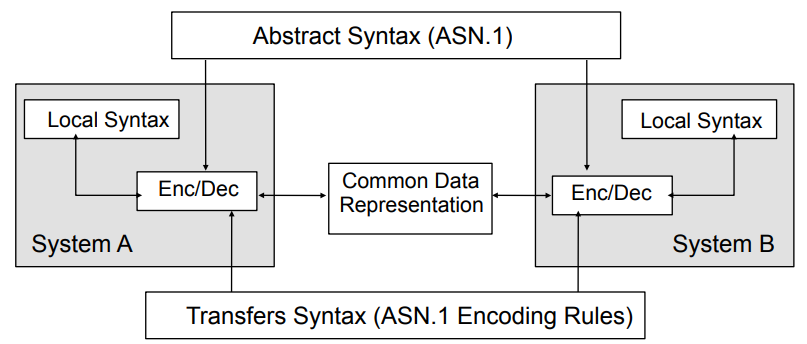
\includegraphics[scale=0.7]{asn1.png}
\end{center}
La sintassi locale (\textbf{local syntax}) è diversa e tipicamente dipendente dal linguaggio utilizzato: ad esempio una in GO l'altra in C, ma anche per sistema A Arduino Nano e sistema B workstation Windows.\\
L'ASN1 quindi definisce una sintassi astratta standardizzata. Permette diverse regole di codifica che trasformano la sintassi astratta in un flusso di byte adatto al trasferimento: \textbf{BER} (Basic Encoding Rules) definisce il mapping tra sintassi astratta e sintassi di trasferimento.\\
ASN1 rimane architettura, idea. La sintassi di trasferimento può essere JSON, GO o qualsiasi altra cosa: l'\textbf{importante è che le due applicazioni si capiscano}.
\begin{list}{}{I \textbf{tipi di dato} (datatypes) primitivi dell'ASN1 sono:}
	\item \texttt{BOOLEAN}
	\item \texttt{INTEGER}
	\item \texttt{BIT STRING}
	\item \texttt{OCTET STRING}
	\item \texttt{OBJECT IDENTIFIER}\\
	Quando trasferisco dati da applicazione ad applicazione, devo poter indicare un campo chiave. Questo tipo di dato identifica univocamente l'oggetto che sto trasferendo all'interno dell'albero ISO
	\item \ldots
\end{list}
\pagebreak
\paragraph{ISO Registration Tree} Usato per identificare univocamente definizioni, documenti, oggetti\ldots Ha una struttura gerarchica, simile ai file system gerarchici. Tutti i nodi di un livello sono univocamente identificati da un numero. Il \textbf{percorso dalla radice al nodo} fornisce una \textbf{sequenza numerica} chiamata \textbf{Object Identifier}.\\
Per esempio, Internet è 1.3.6.1
\begin{center}
	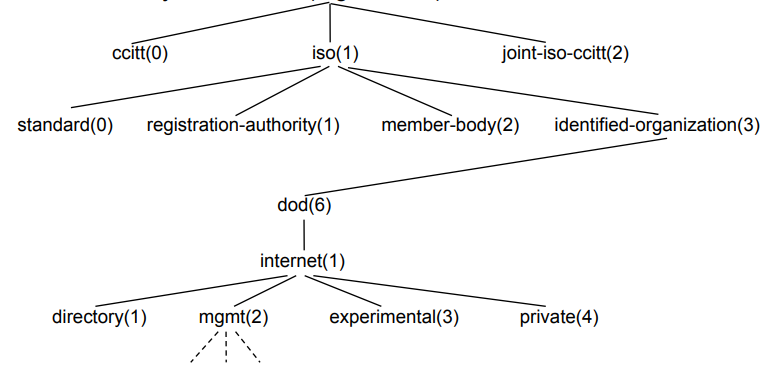
\includegraphics[scale=0.7]{isotree.png}
\end{center}
\textbf{Internet} si trova sotto il \textbf{Dipartimento della Difesa}, che è una \textbf{Organizzazione Identificata} facente parte dell'\textbf{ISO}. Noi parleremo della \textbf{Gestione} (\textbf{m}ana\textbf{g}e\textbf{m}en\textbf{t}) di Internet.\\
L'\textbf{object identifier} quindi, ovvero la sequenza di numeri, risolve il problema dell'identificazione univoca della tipologia dell'oggetto trasmesso sulla rete.
\paragraph{Tipi Complessi} ASN1 ha anche tipi complessi, come \texttt{SEQUENCE OF} che specifica una lista di dati omogenei, o \texttt{REAL} che specifica i numeri reali con mantissa ed esponente dagli \texttt{INTEGER}.
\paragraph{Basic Encoding Rules} Regole di codifica, compattano i dati in una stringa di byte da spedire sul filo. Basato su un algoritmo tag/length/value (TLV), dove ogni variabile è identificata da un tag, la lunghezza del valore in byte e il valore di quei byte. Questo permette al ricevente di ricostruire il tipo del messaggio a partire dal flusso di byte ricevuto.
\chapter{Gestione di Rete}
\section{Nascita}
Gestione di rete nacque, storicamente, nel mondo della telefonia. Necessità di codificare numero, connettersi al centralino, riconoscere il numero\ldots. Standardizzazione necessaria per poter far telefonare a distanze elevate, attraverso le nazioni.
\paragraph{Dati} Poi arrivò internet. Prima bisognava instradare la voce, ora vanno istradati i dati (anche voce, \texttt{VoIP}, ma pur sempre dati). Eredità di tutte le tecnologie e teorie dei tempi della telefonia (es. 5G) ma anche innovazione (es. Browser Web) ma mantenendo il paradigma che era tutto sommato efficiente.
\section{Gestione di Rete Internet}
\paragraph{Cos'è} Sistema di protocolli e tecnologie che permettono di mettere in funzione e controllare un'infrastruttura di rete, per far sì che sia efficiente e che faccia ciò che voglio e che segnali eventuali problemi e comportamenti non previsti.
\paragraph{Reti Geografiche} Questo discorso si applica a reti geografiche, ampie e complesse, che interconnettono un elevatissimo numero di device. Serve anche per far sì che la connessione/disconnessione di dispositivi non crei problemi, e che un utente della rete non possa creare disservizi e potenzialmente tirarla giù.
\paragraph{Anni '90} Il problema principale era mantenere bassi i costi, perché doveva essere pervasivo e poter mettere router in ogni casa. Centraline telefoniche, al contrario, non devono stare in ogni casa.\\
Gli apparati di rete quindi devono costare poco, perciò la gestione di rete non deve costare tanto (nella telefonia costa tanto ed è complicata, quindi "\textit{non facciamo lo stesso errore}": se è semplice anche il costo computazionale è basso, quindi il dispositivo è più economico). Il protocollo, quindi doveva essere \textbf{semplice} e \textbf{efficiente}.\\
Altra cosa importante era \textbf{l'ubiquità} del protocollo: doveva essere disponibile su tutti i dispositivi, così da poterli gestire tutti.\\
Inoltre il protocollo doveva essere \textbf{estensibile}. Almeno \textbf{retrocompatibile}.
\section{SNMP}
\paragraph{Piccoli passi} Il protocollo SNMP è stato progettato di pari passo con il diffondersi di internet, prima a livello universitario e poi industriale. Si è iniziato a sviluppare questo protocollo di gestione dagli albori, perché sin da subito è apparso chiaramente l'importanza che l'infrastruttura stia in piedi.\\
L'SNMP monitora lo stato della rete, per far si che la rete risponda alle esigenze. Ci sono più standard, con primi sviluppati nel 1990.
\paragraph{Semplice} Doveva essere \textbf{semplice}, poiché i sistemi erano semplici, poco potenti e a volte nemmeno multitasking. L'SNMP non poteva girare "in hardware", ma \textbf{necessita di un computer perché necessita di elaborazione dati} e dello stack IP per comunicare. Negli anni '90 lo stack IP non era necessariamente presente sui computer in commercio.\\
La parte importante è che sia \textbf{semplice} e funzionare sotto l'UDP, che è un protocollo estremamente semplice.
\paragraph{Separato} La parte dell'SNMP \textbf{è separata dalla parte di comunicazione} anche se aiuta l'instradamento. \textbf{Non interferisce}, come il cruscotto della macchina (SNMP) col motore (switching).
\paragraph{Trasparente} Sta fuori dalla comunicazione, ma \textbf{deve poterla controllare} e monitorare \textbf{senza interferire}. L'idea è che se l'SNMP viene compromesso lo switch continua a funzionare.
\paragraph{Evoluzione} Nel 1990 viene standardizzata una versione molto semplice: l'\textbf{SNMPv1}. Questa versione fu prodotta in fretta, concentrandosi sulle funzionalità base, in modo da poter entrare subito sul mercato che stava per esplodere.\\
Nle 1991 viene pubblicata la \textbf{Management Information Base}, ovvero l'insieme degli oggetti manipolati tramite l'SNMP.\\
Negli anni successivi ci sono varie evoluzioni del protocollo:
\begin{list}{}{}
	\item \textbf{SNMPv1} supportata da tutti i dispositivi sul mercato
	\item \textbf{SNMPv2} aggiunge poche funzionalità, ma è molto usata soprattutto perché i contatori ora sono a 64bit
	\item \textbf{SNMPv3} aggiunge parecchie funzioni, sacrificando il "\textbf{simple}", quindi non è particolarmente diffuso
\end{list}
\paragraph{Utile} L'SNMP è quindi utile per il monitoring centralizzato su reti estese: è \textbf{importante che questi protocolli siano in funzione in ogni momento}, per riconoscere i problemi in anticipo e avere uno storico della rete per poter fare le verifiche. Anche solo contare il traffico prodotto in termini di byte è un'informazione molto importante.
\paragraph{Agent} \textbf{Apparato di rete}, ad es. nella rete del Fibonacci ci sono diversi agent: access point, computer, stampanti\ldots\\
Sono gli \textbf{oggetti da gestire} e possono cambiare nel tempo: possono essere aggiunti/rimossi, ma possono anche cambiare in tipologia
\subsection{Trap Directed Polling}
Tutti gli agent rispondono ad un manager (solitamente ridondato) $\rightarrow$ $n$ manager per un solo agent.
\begin{center}
	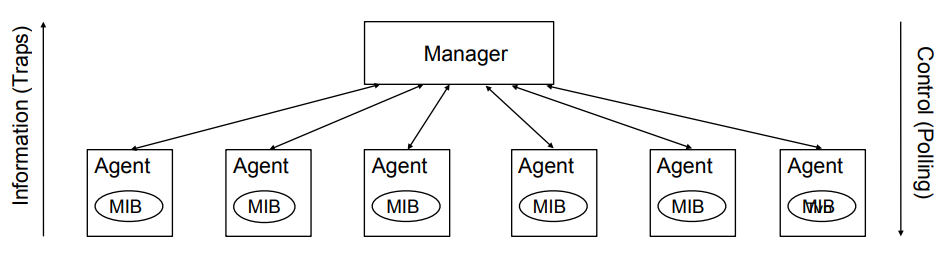
\includegraphics[scale=0.7]{manageragent.png}
\end{center}
\paragraph{Uguaglianza} Con lo stesso protocollo e la stessa funzionalità, devo \textbf{poter controllare dispositivi anche molto diversi}: computer, stampanti, badge, schermi\ldots\\
L'SNMP \textbf{non distingue i dispositivi}, ma \textbf{prende le info dalla MIB} del singolo agent. Ciò che differenzia i vari sistemi operativi, i dispositivi tra loro ecc. sta tutto nella \textbf{MIB} (Management Information Base).
\paragraph{Polling} Controllo. Il manager non comunica continuamente con gli agent, ma esegue un \textbf{polling degli agent}, contattandoli periodicamente per \textbf{ricevere le informazioni aggiornate}.\\
L'SNMP è altamente centralizzato, quindi è compito del manager implementare tutta la funzionalità di monitori e la responsabilità, sicurezza ecc\ldots
\paragraph{Traps} Una volta configurata, sta alla \textbf{periferica avverte il manager se qualcosa non sta funzionando come previsto}. Non informa il manager ogni volta che succede qualcosa (stampo un foglio, prendo un caffè, mi connetto all'Access Point\ldots) perché il manager verrebbe inondato di informazioni, ma \textbf{l'apparato informa il manager se ci sono cose che non funzionano}. Segue la filosofia del "\textit{Se non mandi niente va tutto bene}".\\
Questo può non essere sufficiente, per esempio in caso di problema di rete la comunicazione può non andare a buon fine. In tal caso il polling può risolvere questa cosa, anche se ciò significa apprendere il verificarsi del problema in maniera non tempestiva.
\paragraph{SMI} La struttura delle informazioni di gestione (\textbf{Structure of Management Informativo}, la seconda versione) si basa su un sottoinsieme dei datatype ASN.1 più altri sottotipi:
\begin{list}{}{}
	\item  \texttt{Integer32} interi con il segno
	\item \texttt{Unsigned32} interi senza segno
	\item \texttt{Gauge32} per misure pronte comprese tra min e max
	\item \texttt{Counter32} e \texttt{Counter64} per i contatori: per conoscere la misura effettiva devo fare la differenza tra il valore assunto in due istanti separati.
	\item \texttt{IpAddress} per IPv4
	\item \texttt{TimeTicks} per i centesimi di secondo passati
	\item \texttt{Opaque} che è come il \texttt{void}, non consigliato
\end{list}
Le variabili, inoltre, possono essere
\begin{list}{}{}
	\item \textbf{Scalari}: esistono una sola volta per agent. Es: il nome di un host.
	\item \textbf{Concettuali}: esistono in una tabella concettuale, con valori che cambiano nel tempo.
	\item \textbf{Read} o \textbf{write}, lette o scritte. Non esistono incrementi o reset a valori iniziali, questo per semplicità di protocollo
\end{list}
\paragraph{MIB} Le MIB di SMIv2 sono \textbf{definite tramite speciali macro ASN.1}
\paragraph{Use Case} 
\begin{center}
	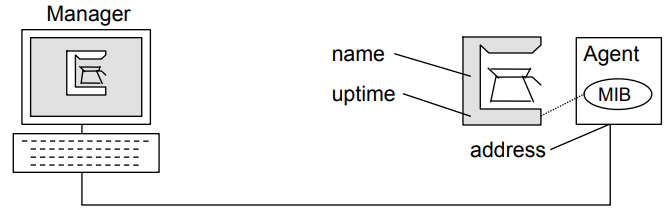
\includegraphics[scale=0.7]{mibusecase.png}
\end{center}
Le variabili sono definite nell'ISO Registration Tree. Una foglia dell'albero rappresente on managed object.
\begin{center}
	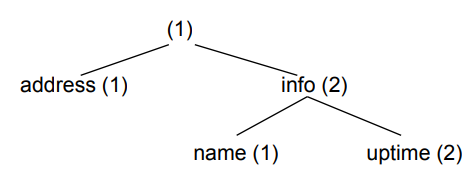
\includegraphics[scale=0.7]{mibusecasetree.png}
\end{center}
\paragraph{Instance Identifier} Ogni managed object è identificato dall'object identifier. Ma tale oggetto ha istanze con determinati valori che cambiano nel tempo: tale istanza è identificata univocamente da un \textbf{Instance Identifier}. La singola istanza di un managed object è \textbf{univocamente identificata concatenando l'Instance Identifier all'Object Identifier}.\\
Gli scalari hanno una sola istanza, e l'istance identifier è \texttt{.0}. Negli altri casi (non identifier) si parte da \texttt{.1}.\\
L'istance identifier è il valore della colonna indice.
\begin{center}
	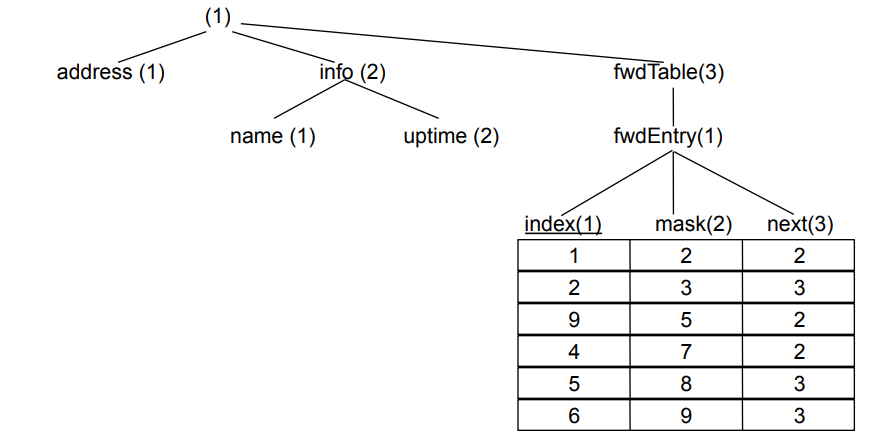
\includegraphics[scale=0.7]{mibusecasetable.png}
\end{center}
In questo caso, per prendere il valore della terza istanza di \texttt{mask}: \texttt{1.3.1.2.9} $\rightarrow$ \texttt{5}.
\begin{multicols}{2}
\begin{list}{}{Altri esempi:}
	\item \texttt{1.3.1.1.1} $\rightarrow$ \texttt{1}
	\item \texttt{1.3.1.2.1} $\rightarrow$ \texttt{2}
	\item \texttt{1.3.1.3.1} $\rightarrow$ \texttt{2}
	\item 
	\item \texttt{1.3.1.1.4} $\rightarrow$ \texttt{4}
	\item \texttt{1.3.1.2.4} $\rightarrow$ \texttt{7}
	\item \texttt{1.3.1.2.7} $\rightarrow$ $\not\exists$
\end{list}
\end{multicols}
\subsection{MIB}
Come si definisce un MIB
\begin{verbatim}
nome DEFINITIONS ::= BEGIN

IMPORT	MODULE-IDENTITY, OBJECT-TYPE, enterprises, IpAddress, TimeTicks	FROM SNMPv2-SMI;
...

END
\end{verbatim}
I nomi servono solo per gli umani, perché sulla rete passano gli object identifier.
\paragraph{Module Identity} Non aggiunge informazione ma indica la versione, questo perché negli anni le reti cambiano ma l'infrastruttura rimane fissa almeno in parte. I device a lungo termine (ad esempio lettori di badge) devono convivere con i nuovi: eterogeneità nelle velocità di elaborazione, protocolli\ldots\\
Non posso togliere oggetto, perché magari versioni precedenti lo usano. Se voglio eliminarlo posso indicarne lo \texttt{STATUS}: obsolete, current o deprecated.
\paragraph{Object Type} \texttt{nome OBJECT-TYPE, SYNTAX, UNITS}\ldots
\paragraph{Notification Type} Invio anche oggetti interessati alle trap\\
linkDown per segnalare se ha perso il link, linkUp per collegamento preso
\paragraph{Utilità dei MIB} Compilatore non è detto che generi linguaggio macchina ma trasforma semplicemente. I \textbf{frontend compilers} SNMP prendono i MIB e producono warning/errori e conversioni di formato SMI
%http://luca.ntop.org/sgr2018/slides/nm2017.pdf
Quando è nato snmp fatti due standard: snmp e mib iniziale (mib-ii, rfc 1213) dove vengono descritti object più importanti per gestione internet.\\
Vogliono controllare stack TCP/IP per vedere cosa non funziona poi monitorare porta di rete. device espongono contatori per interfaccia tramite snmp. contatori byte pacchetti sono base del monitoraggio, ma nel tempo và superato perché contatori su byte sono poco utili: non si sa bene cosa succede però. \\
Obiettivi mib-ii: info base su errori, pochi e semplici control objects (su/giù, errori, pacchett/byte ingresso/uscita), cerca il più possibile di evitare info ridondanti, \textbf{non deve assolutamente interferire con le operazioni} devono essere separati e non rallentare o inficiare in nessuna maniera prestazioni dei dispositivi. Sono circa 170 oggetti, negli anni alcune def sono troppo semplici, e presuppone IPv4 (IPv6 gestito in mib separati).\\
\begin{center}
	schema dei MIB-II (1.3.6.1.2)
\end{center}
\paragraph{Composizione} Diviso in gruppi: \ldots\\
La parte trasmissione è aperta, tanti sottoalberi: com'è connesso computer dipende dalla tecnologia\ldots quindi è estendibile a seconda delle nuove tecnologie\\
Quindi negli anni viene modificato ma è integro sin dalla nascita.\\
Per info più specifiche ci sono mib successivi.
\begin{center}
	tabella
\end{center}
Statistiche su stessa rifa sono a livello diverso, repeater a livello 1. Fanno stessa cosa ma livelli diversi.\\
Per navigare tabelle necessità meccanismo efficiente rispetto a fare tante richieste. Questo perché sistemi modulari, per vedere se valore/elemento esiste.
\paragraph{Ordine lessicografico} Walk:lettura consecutiva di oggetti in mib.\\
Leggo oggetti e metto ordinati per numero in ordine lessicografico. Con questo ordinamento si perde la struttura della tabella: \textbf{SNMP lavora solo su questo array ordinato}.
\paragraph{Trap} Maniera asincrona per informare manager di qualche avvenimento, tipicamente un cambio di stato.\\
\texttt{ifAdminStatus} su \texttt{linkDown} equivale proprio a scollegare fisicamente la scheda di rete. L'\textbf{administrative} è il ciclo di vita, l'\texttt{operational} è operativa. \texttt{ifOperStatus} su \texttt{linkDown} è lo stato e significa che la connessione è caduta.
\subsection{Primitive}
Due tipi di valori, scalari e tabellari.
\paragraph{Get} Richiesta diretta e precisa di un object identifier\\
Può essere usato per leggere una o più variabili. Basato su UDP, quindi dimensione massima pacchetto: nella risposta bisogna stare attenti alle info. Possibile errore (\textbf{errorStatus)}: tooBig, non entra la risposta nel pacchetto UDP. Altri errori: noSuchName (istanza non esiste o non è foglia, esempio chiedere bicchierini ad una stampante), genErr (qualsiasi altro errore: comunità sbagliata, agent sovraccarico\ldots).\\
\textbf{errorIndex} indica quale delle variabili ha avuto problema. Es \texttt{noSuchName@1} indica che la prima variabile non esiste. Posso fare get con più richieste, quindi errore può essere su altra variabile (es \texttt{noSuchName@3} cioè non esiste il terzo object identifier richiesto ma indica il primo indice fallito, quindi le altre due precedenti esistono ma non vengono ritornati i valori).
\paragraph{GetNext} Richiesta che ritorna l'object identifier successivo a quello chiesto.\\
Non legge istance identifier richiesto ma ritorna il prossimo istance identifier rispetto all'ordine lessicografico. usata per fare discovery delle strutture e leggere le tabelle.\\Nella getNext, nosuchname significa che è finito il MIB (non esiste il successivo). Molto implementation depended, alcuni dopo l'ultimo ritornano il primo invece che noSuchName.

\paragraph{Set} Scrivere un valore\\
Equivalente in sostanza alla get ma scrivo. Atomica: più valori sono scritti contemporanemante, quindi o vanno bene tutti o non scrivo niente.\\
Errore \textbf{badValue} quando valore scritto è del tipo sbagliato, fuori dal range o comunque non accettabile. Ma anche errore quando oggetto è \texttt{read-only}.\\
noError quando tutto ok, noSuchName quando instance identifier non esiste. Anche qua stesso discorso della get con l'indice.
\paragraph{Trap} Trap dall'agent\\
\textbf{Unico messaggio non richiesto che va dall'agent verso il manager}.\\
Può succedere trap storm, esempio dopo perdita alimentazione tutti dispositivi segnalano riavvio apparati tutti insieme. Se tolgo corrente non posso fisicamente mandare trap, per questo succede quando riavvio e torna su, non quando va giù tutto insieme.\\
Non ci si può fidare totalmente della trap, bisogna fare polling.\\
\texttt{ColdStart}/\texttt{WarmStart} inviate quando avvio un agent (cold da freddo, spento, caso tipico, invece warm è da riavvio)\\
\texttt{LinkDown}/\texttt{LinkUp}\\
\texttt{AuthenticationFailure} quando faccio richiesta posso non avere autorizzazioni, trap segnala al manager della situazione (tipicamente se provo tante password una dietro l'altra).\\
\texttt{EnterpriseSpecific}, vedi valore enterprise e specific nel formato del pacchetto. ad esempio fine carta di una stampante. Specific=1 per dire che l'interpretazione è a seconda del mib.
\begin{center}
	Formato pacchetti
\end{center}
Community: una sorta di password, vedo se utente che richiede è abilitato a certa operazione. PDU payload data unity\\
Get getnext e set ricevono getresponse tutte e tre.\\
Importante sapere IP host che manda trap (potrebbe vederlo dal pacchetto UDP), perché l'ip nell'udp può essere mascherato o cambiato ad esempio dal nat
\end{document}